\section*{Periodicity}

\subsection*{DFT Assumptions}

We have discussed at length how two sinusoids of different frequencies are orthogonal, assuming they
are both periodic along some interval.  This was a key assumption that allowed us to parse a signal into 
its various constituent frequencies.  Recall that any signal can be broken down into a summation of sinusoids,
and that the inner product is distributive.  
Therefore taking the inner product of some signal $x[n]$ with
a sinusoid $s$ is the same as taking the inner product of $s$ with each sinusoid that
constitutes $x[n]$.  Everything that we have learned so far has hinged on the assumption that all sinusoids, 
including the ones that make up $x[n]$, are periodic along that same interval of samples $N$.  

If you look back
at the small example from earlier, the signal $x[n]$ was composed of two sinusoids $0.5\sin(2\pi t + \pi)$
and $0.25\sin(4\pi t - 1)$, both of which are periodic over one second.  When we took the DFT of that signal,
we tested $x$ for frequencies of 0Hz, 1Hz, 2Hz, etc., all of which are also periodic over one second.  This
example was contrived to work perfectly within the assumptions of the DFT, namely that both $x[n]$ and
our testing frequencies were periodic over the number of samples from the signal.  

In the real world, we will rarely, if ever, be that lucky.  If we were to take a series of $N$ samples from a song
or a speech, it is very unlikely that the slice of audio would be periodic along $N$.  So what are we to do?  Is the
DFT somehow now unusable?  The answer is no.  But we do need to recalibrate our assumptions of what
it can and cannot do.  For one, the DFT will not be able to tell us all the frequencies
and their respective amplitudes and phases with complete precision for any signal.  
The DFT, however, can give us a good \textbf{estimate} of what frequencies are part of some signal.

For a cosine wave that completes exactly $k$ periods, we were able to show precisely what the value of
$X_k$ would be as shown in Equation \ref{eq:complexNumber}.  Though we did not show the derivation for 
that equation, it is similarly
based on the assumption that $x[n]$ is periodic along $N$.  Therefore,
we will not be able to use Equation \ref{eq:complexNumber} for aperiodic $x[n]$.  As a consequence, we 
must also recognize that Equation \ref{eq:amplitude} and 
Equation \ref{eq:phase} will not be able to recover the original amplitudes and phases exactly
 as these are derived from Equation \ref{eq:complexNumber}.  Not all hope is lost
though.  We can still use the DFT to say plenty about the frequency spectrum of $x[n]$.  The magnitude of 
$X_k$ will give us a good estimate of the relative strength of the frequency components in the original 
signal as we will see shortly.  

Some of our conclusions will remain the same regardless of the periodicity of $x[n]$.  The symmetry we saw 
in the magnitude and phase spectrum still applies.  We shall also see that we can perfectly recover the 
original $x[n]$ regardless
of its periodicity using a technique called the Inverse Discrete Fourier Transform.

Though the DFT has shortcomings and does not give the complete picture of the frequency domain for
all $x[n]$, it is still incredibly powerful and useful.  We will still be able to gain a tremendous amount of
information about our signal and do some interesting spectral processing to create engaging audio effects.

\subsection*{DFT of an Aperiodic Sinusoid}

Let us consider what happens when we take the DFT of a signal that is not periodic along $N$.  For ease, let us
start with the simplest of signals, a sinusoid.  We will take $N = 32$ samples from a cosine wave 
that is not periodic along $N$.  The frequency of the cosine wave will be 2.7Hz with an amplitude of 0.5 and a phase of
2.  To get the samples, we can use $x[n] = 0.5\cos(2\pi (2.7)Tn + 2)$ and compute the values for 
$n = 0, 1, 2,...$ etc.
The sampling rate is 32Hz (and thus $T = 1/32$) 
which means we will produce frequency bins of 0Hz, 1Hz, 2Hz, etc.  Importantly, note that there is no frequency bin 
for 2.7Hz.  

\begin{figure}[h]
	\caption{The time domain, magnitude and phase spectra of $x[n] = 0.5\cos(2\pi (2.7)Tn + 2)$
	for $N = 32$ and $f_s = 32$Hz.}
	\label{fig:aperiodicGraph}
	\begin{center}
		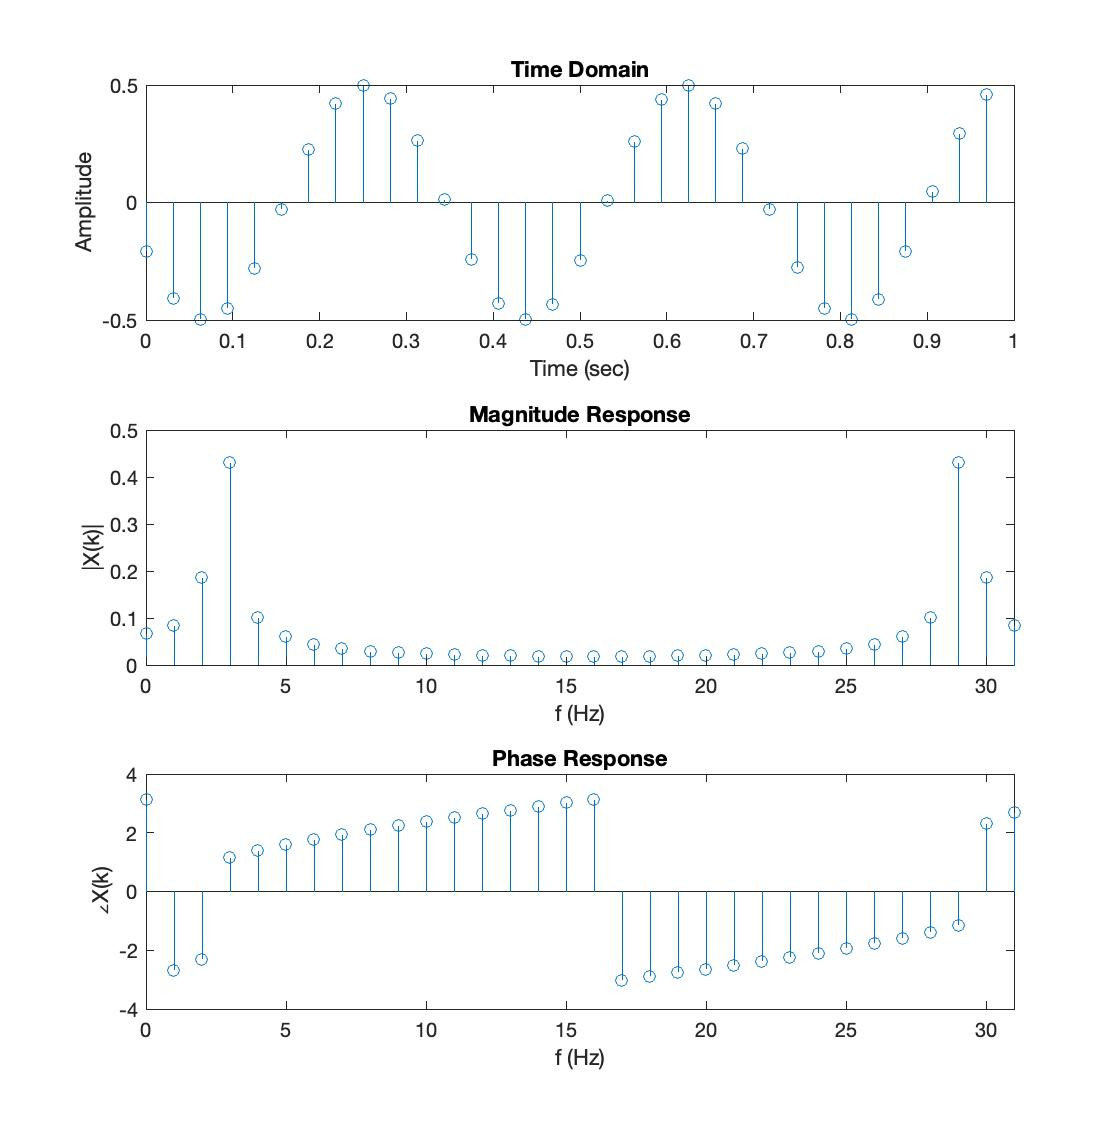
\includegraphics[scale = 0.3]{aperiodic.jpg}
	\end{center}
\end{figure}

Plotted in Figure \ref{fig:aperiodicGraph} is the magnitude and phase spectra of the original signal as well as its time 
domain representation because the signal does not complete an even number of cycles.  It completes
two complete cycles plus some fractional number of cycles.  After computing the DFT of $x[n]$, Figure 
\ref{fig:aperiodicGraph} shows the magnitude and phase spectra.
The magnitude spectrum was calculated by taking the magnitude of each complex number.  
If we look at the graph, we can see two peaks roughly between 2 and 3Hz
and between 29 and 30Hz.  We can also see the symmetry between the two halves if we split the magnitude spectrum
down the middle.  We can see that every frequency bin has some magnitude in it which might suggest that our original
signal was composed of 32 sinusoids of varying amplitudes.  But we know that is not the case.  There is just one at
2.7Hz.  We can, however, see ``activity" at 2.7Hz in the magnitude spectrum due to the peak at that point.  The other peak
is simply the mirror image of 2.7Hz above the Nyquist frequency.  We saw this symmetry occurred even with periodic
sinusoids.  So many of the same instincts that we derived in the context or periodic $x[n]$ hold true with aperiodic 
$x[n]$. 

How do we account though for positive magnitudes in all the bins?  This is a phenomenon called \textbf{spectral leakage}.  
We will always see peaks in the magnitude spectrum at the frequencies of $x[n]$ provided those frequencies have
sufficient amplitude.  Notice though that each frequency bin registers some level of magnitude.  Farther away from the 
peak, the magnitudes decrease but are still non-zero.  This is called ``spectral leakage".  It is important to understand
that we are not seeing multiple frequencies.  Rather we are seeing the effect of how one aperiodic component of $x[n]$
spreads out to all frequency bins.   

Can we recover the original amplitude of 0.5 from the magnitude spectrum?  The answer, in short, is no.  For one, we
would need to guess about where the apex of the peak was.  The peak is always centered at the frequency of each
component of $x[n]$.  It is hard to tell based on the magnitude spectrum though where exactly that is.  We can use
a process called interpolation to estimate the peak.  Even so, each frequency component of $x[n]$ spreads to each
adjacent bin.  Therefore, even if we could determine the peak, the magnitude at that location could be the product
of the spread of several different peaks.  Therefore, it will be impossible to reconstruct the original amplitude.  
Nevertheless we can get a good sense of the relative strength of each component.  Higher peaks represent stronger
frequency components; lower peaks represent weaker frequency components.

How can we interpret the phase spectrum?  Again we see a sudden change around 2Hz.  The phase spectrum shifts
drastically at the location moving from negative to positive.  The original phase of the sinusoid from $x[n]$ was $+2$,
and it is hard to see any relationship between the phase spectrum of $x[n]$ around 2.7Hz and the original phase.  In 
general, the phase spectrum of the DFT is more abstruse and difficult to parse.  Sometimes sudden shifts in the
phase spectrum are the result of the periodic nature of sinusoids.  Phases outside the range $+\pi$ to $-\pi$ get
wrapped back down to that range.  This can cause abrupt shifts in the phase spectrum.  We will not be spending
much time examining the phase spectrum as it usually is less important for musical applications. We shall see soon
though that there is a better way to interpret the phase spectrum.

\subsection*{The Periodicity of the DFT}

We have seen how the DFT responds to periodic and aperiodic sinusoids.  In this section, I would like to offer 
another perspective on the DFT.  We have learned that the DFT can accurately parse the frequencies of $x[n]$ if
$x[n]$ is periodic along those $N$ samples.  I should also state explicitly that the DFT \textbf{assumes} that
those $N$ samples are from a periodic function regardless of whether they are or not and that those $N$ samples
constitute a period from that periodic signal $x[n]$.  

If we look back at the time
domain representation of Figure \ref{fig:aperiodicGraph}, we can see a plot of the samples from the sinusoid of
2.7Hz.  The DFT assumes those $N$ samples make up one period of the periodic signal $x[n]$.  $x[n]$
is indeed periodic but those $N$ samples are not a period of $x[n]$.  One way to see what the DFT ``sees" is to
simply repeat those $N$ samples and look at the time domain representation of the sound.  The top plot in Figure
\ref{fig:basis} shows a plot of 2.7Hz with more samples to highlight the disjointed transition when the samples
repeat.  Importantly, the DFT is parsing the frequencies of this signal and not the smoothly oscillating sinusoid 
from where the samples originated.  The abrupt transition that happens at each repeat creates an entirely new signal.  
That is the signal that the DFT converts to the frequency domain, and accurately I might add.  Another way, then,
to think about spectral leakage is that it is the distortion of the original waveform that occurs when we fail
to capture a complete period.  An important intuition to take away is that sharp discontinuities in the time domain
create rich spectrum in the frequency domain.

In math, we can show that nearly all periodic signals can be
represented as a sum of cosine waves where each cosine wave is a harmonic of the fundamental period $N$.\footnote{I
mention ``nearly all" because such a signal must satisfy the Dirichlet conditions.  But for all pratical purposes, any
real audio signal will satisfy the Dirichlet conditions.}  
This is called the Fourier Series, and it turns out we can derive the DFT from the Fourier Series.  We will not
do that here.  But the main point is that the DFT assumes the $N$ samples are a period from periodic $x[n]$ and 
attempts to
represent the $N$ samples as a sum of cosine waves, each of which is a harmonic of the period $N$.  

To demonstrate the Fourier Series, we will use a classic example: the square wave.  The Fourier Series tells us we
can represent the square wave as a sum of cosine waves.  This should feel wrong on some intuitive level.  The
square wave has discontinuities and lines of zero slope.  It would seem impossible that we could take a series of
cosine waves -- let alone cosine waves from a harmonic series -- and sum them to create a square wave.  Yet it is 
true!  A square
wave can indeed be created by summing the odd harmonics where each harmonic's amplitude is one over 
the harmonic number.

Figure \ref{fig:square} shows an iterative process where each successive chart shows the next harmonic 
added.  As more and more harmonics get added, the graph begins to move closer to the shape of a square wave.  A
square wave is composed of an infinite number of harmonics.  So we will not be able to display the sum of an infinite
number of sinusoids using a computer.  This example though illustrates a key point of signal processing, namely that any
periodic waveform can be represented as a sum of harmonic sinusoids.  

\begin{figure}[h]
	\caption{Successive addition of harmonics to approximate a square wave}
	\label{fig:square}
	\begin{center}
		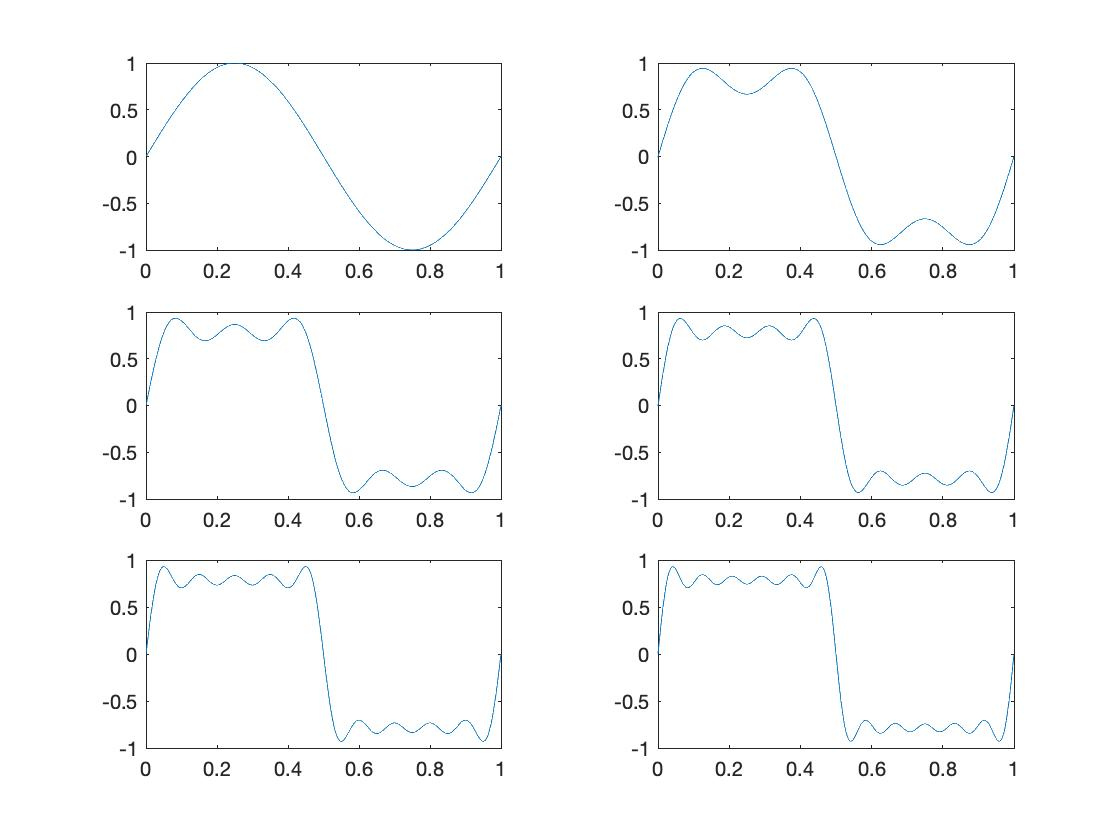
\includegraphics[scale = 0.3]{square.jpg}
	\end{center}
\end{figure}

\begin{figure}[h]
	\caption{Periodicity of the DFT as shown through the time domain representation in the samples and the cosine basis}
	\label{fig:basis}
	\begin{center}
		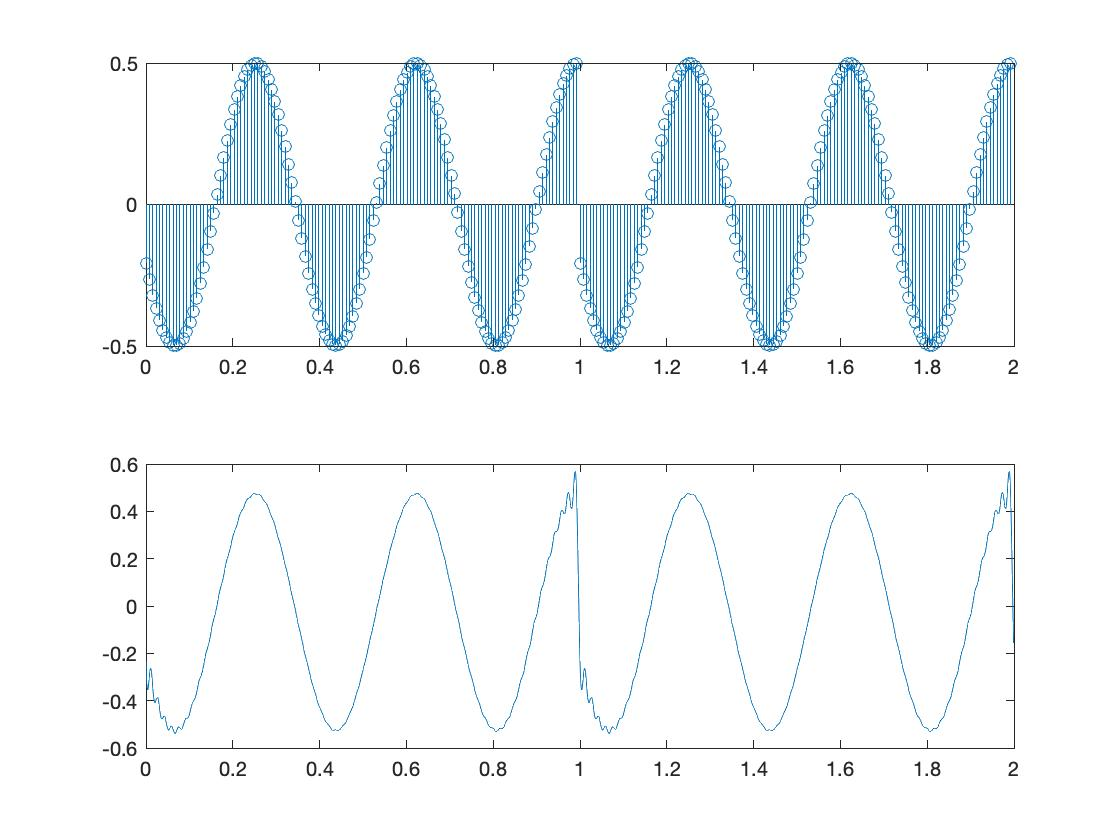
\includegraphics[scale = 0.3]{basis.jpg}
	\end{center}
\end{figure}

Let us look back at the example we used to discuss how the DFT reacted to an aperiodic sinusoid.  In that example,
we took a slice of $N = 32$ samples from $x[n] = 0.5\cos(2\pi (2.7)Tn + 2)$ that did not capture a complete period
from $x[n]$.  Nevertheless, the DFT still considered those $N$ samples to be periodic.  Again, the top
plot in Figure \ref{fig:basis} shows how the DFT perceives the periodicity of that waveform.  
Because that signal is periodic, we can represent it using a sum of harmonic cosine waves.  The bottom plot from 
Figure \ref{fig:basis} shows an approximation of that signal with a sum of harmonic cosine waves.  How did I know 
which cosine waves to sum to achieve this approximation?  From the DFT, of course!  \textbf{Another interpretation of the
DFT is that it encodes the information to recreate the original signal using a sum of cosine waves.}


The magnitude and phases we calculate for each frequency bin
can be used in conjunction with the frequency of each bin to construct a series of cosines waves that,
when summed, produce the approximation shown in the bottom plot from Figure \ref{fig:basis}.\footnote{Note that 
we will be using a normalized magnitude here where the magnitude of the complex number $X_k$ is multiplied by
a factor of $2/N$.}  For example,
the first frequency bin has a frequency of 0, magnitude of 0.0523, and a phase of $\pi$.  If we plug those values 
into a cosine wave, we get $0.0523 * \cos(2 * \pi * 0 * t + \pi) = 0.0523 * (-1) = -0.0523$.  The first frequency bin
of every DFT is always how much DC offset is in the signal.  We can see that $-0.0523$ is relatively small which 
makes sense because our original signal, even lopped off at the end, has relatively little DC offset.  The second
 frequency bin has a frequency of 1Hz, a magnitude of 0.0696, and a phase of $-2.6026$.  If we plug those values into
 a cosine wave, we get $0.0696 * \cos(2 * \pi * (1) * t - 2.6026) = 0.0696\cos(2\pi t - 2.6026)$.  We can add this to
 $-0.0523$ to get the first two sinusoidal approximation.  If we continued in this fashion with every frequency bin
 up to $k = N/2$, the Nyquist frequency, we get the approximation shown in the bottom plot from 
 Figure \ref{fig:basis}.  
 
 	In this interpretation of the DFT, we can see how both the phase and magnitude derive meaning.  We can think
 of the DFT as producing a series of harmonic cosine waves that get their specific parameters from the values in each
frequency bin.  We call these harmonic cosine waves a \textbf{basis}, and we \textbf{project} our original signal
$x[n]$ onto this basis.  This is the geometric interpretation of the DFT.  The terms ``projection" and ``basis" are 
mathematical terms.  One common ``basis" we all know is the coordinate axis system.  It is a space that allows us
to plot any 2D shape.  A series of harmonic cosine waves also form a basis.  It is a basis that allows us to 
plot or describe any periodic signal.  We can think of projection as a means to transform our original signal
 in terms of our basis (i.e., a sum of cosine waves).  But how exactly do we do this projection
 or transformation?  With the inner product.  The inner product, with which we started our duscussion of the DFT,
 is a means of projecting a signal onto a different basis such as the frequency domain.  Therefore, another way to
 view the DFT is that it takes a period of $N$ samples and projects them onto a set of harmonic sinusoids that
 approximate the waveform described by those $N$ samples.
